% Options for packages loaded elsewhere
\PassOptionsToPackage{unicode}{hyperref}
\PassOptionsToPackage{hyphens}{url}
\PassOptionsToPackage{dvipsnames,svgnames*,x11names*}{xcolor}
%
\documentclass[
]{article}
\usepackage{lmodern}
\usepackage{setspace}
\usepackage{amssymb,amsmath}
\usepackage{ifxetex,ifluatex}
\ifnum 0\ifxetex 1\fi\ifluatex 1\fi=0 % if pdftex
  \usepackage[T1]{fontenc}
  \usepackage[utf8]{inputenc}
  \usepackage{textcomp} % provide euro and other symbols
\else % if luatex or xetex
  \usepackage{unicode-math}
  \defaultfontfeatures{Scale=MatchLowercase}
  \defaultfontfeatures[\rmfamily]{Ligatures=TeX,Scale=1}
\fi
% Use upquote if available, for straight quotes in verbatim environments
\IfFileExists{upquote.sty}{\usepackage{upquote}}{}
\IfFileExists{microtype.sty}{% use microtype if available
  \usepackage[]{microtype}
  \UseMicrotypeSet[protrusion]{basicmath} % disable protrusion for tt fonts
}{}
\makeatletter
\@ifundefined{KOMAClassName}{% if non-KOMA class
  \IfFileExists{parskip.sty}{%
    \usepackage{parskip}
  }{% else
    \setlength{\parindent}{0pt}
    \setlength{\parskip}{6pt plus 2pt minus 1pt}}
}{% if KOMA class
  \KOMAoptions{parskip=half}}
\makeatother
\usepackage{xcolor}
\IfFileExists{xurl.sty}{\usepackage{xurl}}{} % add URL line breaks if available
\IfFileExists{bookmark.sty}{\usepackage{bookmark}}{\usepackage{hyperref}}
\hypersetup{
  pdftitle={Perceptions and Preferences for Meritocracy},
  colorlinks=true,
  linkcolor=blue,
  filecolor=Maroon,
  citecolor=Blue,
  urlcolor=Blue,
  pdfcreator={LaTeX via pandoc}}
\urlstyle{same} % disable monospaced font for URLs
\usepackage{graphicx,grffile}
\makeatletter
\def\maxwidth{\ifdim\Gin@nat@width>\linewidth\linewidth\else\Gin@nat@width\fi}
\def\maxheight{\ifdim\Gin@nat@height>\textheight\textheight\else\Gin@nat@height\fi}
\makeatother
% Scale images if necessary, so that they will not overflow the page
% margins by default, and it is still possible to overwrite the defaults
% using explicit options in \includegraphics[width, height, ...]{}
\setkeys{Gin}{width=\maxwidth,height=\maxheight,keepaspectratio}
% Set default figure placement to htbp
\makeatletter
\def\fps@figure{htbp}
\makeatother
\setlength{\emergencystretch}{3em} % prevent overfull lines
\providecommand{\tightlist}{%
  \setlength{\itemsep}{0pt}\setlength{\parskip}{0pt}}
\setcounter{secnumdepth}{5}

\title{Perceptions and Preferences for Meritocracy}
\author{}
\date{\vspace{-2.5em}}

\begin{document}
\maketitle

\setstretch{1.5}
\hypertarget{introducciuxf3n}{%
\section{Introducción}\label{introducciuxf3n}}

La desigualdad económica se ha vuelto un tema que genera creciente
preocupación y malestar alrededor del mundo. Esto se ha expresado en una
serie de protestas como la emblemática ``occupy wall street'' el año
2011, así como también en una serie de análisis críticos respecto del
desarrollo del capitalismo y sus consecuencias (Piketty
\protect\hyperlink{ref-PikettyCapitalTwentyFirstCentury2014b}{2014}). En
este contexto, el estudio de las visiones, preferencias y percepciones
respecto de la desigualdad han adquirido relevancia en las ciencias
sociales, en temas como las preferencias redistributivas (Alesina and
Angeletos \protect\hyperlink{ref-alesina_Fairness_2005}{2005}; Dimick,
Rueda, and Stegmueller \protect\hyperlink{ref-dimick_Models_2018}{2018})
la legitimación de la desigualdad económica (Schröder
\protect\hyperlink{ref-schroder_Income_2017}{2017}) y el funcionamiento
de la meritocracia (Duru-Bellat and Tenret
\protect\hyperlink{ref-Duru-BellatWhoMeritocracyIndividual2012b}{2012}\protect\hyperlink{ref-Duru-BellatWhoMeritocracyIndividual2012b}{a};
Mijs
\protect\hyperlink{ref-MijsParadoxInequalityIncome2019b}{2019}\protect\hyperlink{ref-MijsParadoxInequalityIncome2019b}{a};
Reynolds and Xian
\protect\hyperlink{ref-ReynoldsPerceptionsMeritocracyLand2014b}{2014}\protect\hyperlink{ref-ReynoldsPerceptionsMeritocracyLand2014b}{a}).

En general, la meritocracia se define como un sistema de distribución de
recursos y recompensas basados en el mérito individual, que en su
concepción original es una suma de talento y esfuerzo (Young
\protect\hyperlink{ref-young_rise_1962}{1962}) y que pone en un lugar
secundario interferencia de factores estructurales como la herencia o
los contactos (Breen and Goldthorpe
\protect\hyperlink{ref-breenClassInequalityMeritocracy1999}{1999};
Saunders \protect\hyperlink{ref-saundersMightBritainBe1995}{1995}; Yair
\protect\hyperlink{ref-yairMeritocracy2007}{2007}; Land
\protect\hyperlink{ref-landWeSatTable2006}{2006}; Young
\protect\hyperlink{ref-youngRiseMeritocracy1994}{1994}). Una serie de
estudios han realizado críticas a la realización de este estándar moral
de distribución, planteando que es una promesa incumplida dada la
influencia preponderante de otros elementos más allá del mérito en el
estatus individual (Witteveen and Attewell
\protect\hyperlink{ref-WitteveenReconsideringmeritocraticpower2020a}{2020};
Arrow, Bowles, and Durlauf
\protect\hyperlink{ref-arrow_meritocracy_2000}{2000}; Goldthorpe
\protect\hyperlink{ref-goldthorpe_myth_2003}{2003}; Markovits
\protect\hyperlink{ref-markovits_Meritocracy_2019}{2019}). Por otro
lado, desde la psicología social y la sociología se han estudiado las
características y consecuencias de las creencias en la meritocracia, en
general basados en la hipótesis que mayor creencia en la meritocracia
lleva a una mayor legitimación de las desigualdades (Preminger
\protect\hyperlink{ref-PremingerMeritocracyserviceethnocracy2020}{2020};
Trump \protect\hyperlink{ref-TrumpWhenwhyeconomic2020}{2020}; Meredith
\protect\hyperlink{ref-Meredithsocietydivisibleblessed2020}{2020};
Hadjar \protect\hyperlink{ref-hadjar_meritokratie_2008}{2008}; Madeira
et al.
\protect\hyperlink{ref-MadeiraPrimesConsequencesSystematic2019}{2019}).

Debido al rol que cumplen las creencias meritocráticas dentro del
pensamiento neoliberal (Bay-Cheng et al.
\protect\hyperlink{ref-Bay-ChengTrackingHomoOeconomicus2015}{2015}), han
surgido múltiples investigaciones que evalúan la relación entre
creencias meritocráticas y diversos ámbitos sociales de la actualidad.
Se han desarrollado estudios que vinculan la meritocracia con el
reforzamiento de estereotipos socioeconómicos, de género y de etnias
(Madeira et al.
\protect\hyperlink{ref-MadeiraPrimesConsequencesSystematic2019}{2019};
Girerd and Bonnot
\protect\hyperlink{ref-GirerdNeoliberalismIdeologicalBarrier2020}{2020};
Preminger
\protect\hyperlink{ref-PremingerMeritocracyserviceethnocracy2020}{2020}).
Igualmente, se han desarrollado líneas de investigación que evalúan el
efecto de las creencias meritocráticas en el contexto educativo
(Generett and Olson
\protect\hyperlink{ref-GenerettStoriesWeTell2020}{2020}; Reay
\protect\hyperlink{ref-ReayPerilsPenaltiesMeritocracy2020}{2020}; Owens
and de St Croix
\protect\hyperlink{ref-OwensENGINESSOCIALMOBILITY2020}{2020}). y en el
contexto organizacional de las empresas (Pérez and Sabelis
\protect\hyperlink{ref-PerezAdvancingcareersmerit2020}{2020}; Aiello,
Cardamone, and Pupo
\protect\hyperlink{ref-AielloNewevidencefirmuniversity2019}{2019})

Para poder dar cuenta de los niveles de creencia en la meritocracia los
estudios a la fecha generalmente han utilizado algunos indicadores de
encuestas ya existentes, y en el menor de los casos se han creado
instrumentos ad-hoc. Sin embargo, y como mostraremos más adelante, las
formas de medición de meritocracia varían extremadamente entre estudios.
Muchas veces fenómenos similares se asocian a indicadores distintos, y
también ocurre que fenómenos distintos son medidos con indicadores
similares, todo lo cual hace dificulta la comparabilidad entre estudios
y el poder avanzar en la comprensión del concepto de meritocracia.

Basados en el análisis crítico de las formas de medición de meritocracia
a la fecha, el presente estudio propone un instrumento para medir y
relacionar dos aspectos claves en el estudio de la meritocracia:
percepciones y preferencias. Además, como un segundo eje de análisis
considera la generación de indicadores respecto de aspectos
meritocráticos y anti-meritocráticos, demostrando que no son los dos
polos de un mismo continuo como muchos estudios anteriores parecen
sugerir. La propuesta de medición además está orientada a generar un
instrumento lo más breve posible de manera que pueda ser utilizado en
encuestas de opinión.

\hypertarget{la-mediciuxf3n-de-los-aspectos-subjetivos-de-la-meritocracia}{%
\section{La medición de los aspectos subjetivos de la
meritocracia}\label{la-mediciuxf3n-de-los-aspectos-subjetivos-de-la-meritocracia}}

A continuación se presenta una revisión de una serie de investigaciones
que se han abocado al estudio de la meritocracia y que para ello han
hecho una propuesta de medición. El primer eje de análisis tiene que ver
con el uso del concepto ``creencias'' para referir a distintos aspectos
subjetivos relacionados con meritocracia. El segundo eje tiene que ver
con el uso de indicadores sobre aspectos anti-meritocráticos como el
polo opuesto de los meritocráticos.

\hypertarget{la-caja-negra-de-las-creencias-en-la-meritocracia}{%
\subsection{La caja negra de las creencias en la
meritocracia}\label{la-caja-negra-de-las-creencias-en-la-meritocracia}}

Para ejemplificar la confusión del uso de creencias en meritocracia
consideremos en primer lugar un artículo reciente de Mijs, donde se
expresa la siguiente definición: ``when I discuss meritocracy beliefs, I
am referring to citizens' belief in the importance of hard work relative
to structural factors.'' (Mijs
\protect\hyperlink{ref-mijs_paradox_2019}{2019}\protect\hyperlink{ref-mijs_paradox_2019}{b},
pg.9). In the operationalization, this is associated with the following
indicator: ``how important you think it is for getting ahead in life:
(a) hard work'', scored in a 1 to 5 likert scale. There are several
assumptions behind this decision that are worth discussing:

\begin{enumerate}
\def\labelenumi{\alph{enumi}.}
\item
  Dimensionality: the item used by Mijs is part of an battery present in
  several international surveys usually called ``get ahead'', which
  presents a series of indicators related to what people consider
  important to get ahead in life: hard work, education, ambition,
  wealthy family, right connections, religion, race and gender. For
  Mijs, other aspects as education, that could be associated to talent,
  are not meritocratic: ``Hard work is arguably the most meritocratic
  part of Michael Young's equation, `Merit = Intelligence + Effort', for
  the simple fact that intelligence itself is conditioned by a
  nonmeritocratic factor: who your parents happen to be'' (p.5). This is
  a very strong assumption: effort would not depend on parents
  influence, and talent is not meritocratic. A similar approach only
  considering effort as the main element of meritocracy is taken by
  other authors ho only included effort as an indicator of meritocratic
  beliefs (Maitner
  \protect\hyperlink{ref-MaitnerEmotionalreactionsunequal2015}{2015};
  Major et al.
  \protect\hyperlink{ref-MajorPerceiveddiscriminationworldview2007}{2007};
  Bubak
  \protect\hyperlink{ref-BubakPerceptionsmeritocracynote2019}{2019};
  {\textbf{???}}). We suggest here is that questions such as whether
  talent is not meritocratic (or less meritocratic than effort) should
  be open to empirical scrutiny and not disregarded upfront based on
  scholars' assumptions. Besides, the use of single indicators for
  measurement a construct is based on the assumption of a measurement
  without error.
\item
  Beliefs: the ``get ahead'' battery refers to ``how important you think
  it is'', considered by Mijs as a belief in meritocracy. Nevertheless,
  another version of this same battery asks about ``how important you
  think it \emph{should} be''. Which one of both is the ``belief''? If
  we consider belief as related to a normative content, actually the
  more close version is the ``should be'', being the other one more
  close to the perception of the situation. Such distinction was already
  made by Duru-Bellat and Tenret
  (\protect\hyperlink{ref-duru-bellat_whos_2012}{2012}\protect\hyperlink{ref-duru-bellat_whos_2012}{b}),
  who used the item ``how important should the number of years spent in
  education and training be in deciding how much money people ought to
  earn?'' for ``desired'' meritocracy, whereas for ``perceived''
  meritocracy they use two items: ``Would you say that in your country,
  people are rewarded for their efforts?'' and ``\ldots{} people are
  rewarded for their skills?''. Is the belief in meritocracy a
  perception or a preference? A comprehensive measurement should be in
  line with what Duru-Bellat and Tenret
  (\protect\hyperlink{ref-duru-bellat_whos_2012}{2012}\protect\hyperlink{ref-duru-bellat_whos_2012}{b})
  did, in order to open up possibilities of analyzing whether
  perceptions and preferences are actually the same (i.e.~correlation
  close to 1) or they are different aspects of the same phenomenon.
  Therefore, two main drawbacks of the term ``beliefs'' are that (i) it
  hides different operationalizations of the concept of meritocracy, and
  (ii) it blurs the distinction between perceptions and preferences. We
  argue that perceptions and preferences should be disentangled and used
  together, specially when analyzing preferences. As Son Hing et al.
  (\protect\hyperlink{ref-son_hing_merit_2011-1}{2011}) have pointed
  out, ``People can believe that outcomes ought to be distributed on the
  basis of merit and yet vary in their perceptions of whether this is
  how society currently operates'' (p.~435). In other words, preferences
  should be interpreted in the context of perception: a large preference
  for meritocracy certainly means something totally different for
  someone perceiving high meritocracy than for someone perceiving low
  meritocracy.
\item
  Non-meritocratic aspects: Mijs
  (\protect\hyperlink{ref-mijs_paradox_2019}{2019}\protect\hyperlink{ref-mijs_paradox_2019}{b})
  make reference to some non-meritocratic aspects as talent, letting
  this out of the measurement. A different approach was followed by
  Kunovich and Slomczynski
  (\protect\hyperlink{ref-kunovich_systems_2007}{2007}), who decide to
  include non-meritocratic elements in the measurement of meritocracy.
  Using the items' battery listing a number of reasons about ``How
  important should be in deciding pay\ldots{}'' (as Duru-Bellat and
  Tenret
  (\protect\hyperlink{ref-duru-bellat_whos_2012}{2012}\protect\hyperlink{ref-duru-bellat_whos_2012}{b})
  for desired meritocracy), he decided that reasons as education and
  responsibility are meritocratic and pointed 1 if considered essential,
  whereas reasons such as having a family and children were pointed 1 if
  they were considered ``not important at all'' (i.e.~reverse coded). A
  similar approach was taken by Newman, Johnston, and Lown
  (\protect\hyperlink{ref-newman_false_2015}{2015}), reverse-coding
  non-meritocratic items, similarly to what occurs with the ``Preference
  for the Merit Principle Scale'' (Davey et al.
  \protect\hyperlink{ref-davey_preference_1999}{1999}). The assumption
  that meritocratic and non-meritocratic elements are the poles of the
  same continuum was analyzed by Reynolds and Xian
  (\protect\hyperlink{ref-reynolds_perceptions_2014}{2014}\protect\hyperlink{ref-reynolds_perceptions_2014}{b})
  using the same ``get ahead'' perceptions' battery items. They consider
  education, ambition and hard work as meritocratic and other reasons
  such as wealthy family and right connections and non-mertitocratic.
  Nevertheless, despite making this distinction the author ends up
  substracting one dimension from the other, assuming that they are two
  poles of the same continuum as Kunovich and Slomczynski
  (\protect\hyperlink{ref-kunovich_systems_2007}{2007}) did.
\item
  Accounting for measurement error: finally, most of the studies in
  meritocracy so far have not incorporated the issue of measurement
  error ({\textbf{???}}), using single indicators and/or composite
  indexes for measuring meritocracy. This means assuming that the
  construct is measured perfectly by the indicators chosen, going as far
  as proposing that "we decided to rely on a summative index. In
  choosing this strategy of index construction, we argue that
  \emph{support for meritocracy is not a latent variable} (Kunovich and
  Slomczynski \protect\hyperlink{ref-kunovich_systems_2007}{2007},
  653--54). Some advances were done by Reynolds and Xian
  (\protect\hyperlink{ref-reynolds_perceptions_2014}{2014}\protect\hyperlink{ref-reynolds_perceptions_2014}{b})
  by doing a principal component analysis of meritocratic and
  non-meritocratic dimensions, but somewhat contradictorily they end up
  in a sum index despite proving multidimensionality.
\end{enumerate}

\hypertarget{an-instrument-proposal}{%
\subsection{An instrument proposal}\label{an-instrument-proposal}}

Based on the previous limitations in the measurement of meritocracy
presented in the previous section, in this paper we propose and test an
instrument with the following characteristics:

\begin{itemize}
\tightlist
\item
  Multidimensional, incorporating previous distinctions between
  preferences and perceptions as well as between meritocratic and
  non-meritocratic aspects.
\item
  Multiple indicators for each dimension, in order to account for
  measurement error in a confirmatory factor analysis context.
\item
  Based on previous indicators as far as possible, for the sake of
  comparability between studies
\item
  Brief, as to be used in a regular survey. In this point it differs for
  instance from the proposal of the ``Preference for the Merit Principle
  Scale'' (Davey et al.
  \protect\hyperlink{ref-davey_preference_1999}{1999}), as they use 15
  items just for one dimension (besides the problem of reverse-coding
  non-meritocratic items).
\end{itemize}

The proposed measurement framework is based on two axis of analysis, as
depicted in Table 1:

The first axis distinguishes between different types of ``beliefs'',
using instead the terms perceptions and preferences for meritocracy
(Duru-Bellat and Tenret
\protect\hyperlink{ref-duru-bellat_whos_2012}{2012}\protect\hyperlink{ref-duru-bellat_whos_2012}{b};
Son Hing et al. \protect\hyperlink{ref-son_hing_merit_2011-1}{2011}).
Perceptions refers to the extent to which people see meritocracy working
in their society, which in terms of measurement relates to the ``reasons
to get ahead'' battery, whereas preferences refer to normative
expectations that are usually linked to a ``should'' expression
(e.g.~whether hard work should be related to payment). The second axis
consider the distinction between meritocratic and non-meritocratic
dimensions (Reynolds and Xian
\protect\hyperlink{ref-reynolds_perceptions_2014}{2014}\protect\hyperlink{ref-reynolds_perceptions_2014}{b}).
This aspect has been usually treated as different ends of a same
continuum in part of the previous research, an assumption that requieres
empirical scrutiny. These non-meritocratic elements usually refer to the
use of personal contacts or family advantages to get ahead in life.

Regarding the selection of indicators, most of them some adaptations of
previous items that where streamlined in order to a better fit with the
specific dimensions. For meritocratic indicators we use effort and
talent as the main components of the traditional concept of merit as
defined by Young (\protect\hyperlink{ref-young_rise_1962}{1962}),
whereas for non-meritocratic dimensions we use having rich parents and
good contacts. The description of the specific items is presented in the
methodology section.

\textbf{Hypotheses}

\begin{itemize}
\item
  H1. The perception of meritocracy is a latent variable based on
  indicators of the importance attributed to talent and the effort to
  get ahead in life.
\item
  H2. The non-meritocratic perception is a latent variable that derives
  from two indicators related to the agreement with the statement that
  people with contacts and rich parents manage to get ahead.
\item
  H3. Meritocratic preferences behave as the latent variable based on a
  normative value of effort and talent.
\item
  H4. Non-meritocratic preferences behave as a latent variable based on
  the normative value of the use of personal contacts and having rich
  parents.
\end{itemize}

\hypertarget{methodology}{%
\section{Methodology}\label{methodology}}

\hypertarget{data-collection}{%
\subsection{Data collection}\label{data-collection}}

The data was obtained through an online questionnaire which was part of
a larger study on meritocracy and preferences developed in Chile in 2019
and funded by the national scientific agency FONDECYT. The questionnaire
was programmed in Qualtrics and the fieldwork was in charge of an
external online survey agency
(\href{www.netquest.cl}{netquest.cl})during December 2019 and January
2020. The sample was selected from a non-probabilistic design in three
large cities in Chile. The quota method based on age, sex and
educational level was used. Quotas were generated based on the survey of
the Public Studies Center (CEP, 2019), which has a high prestige in the
country and is also the counterpart agency of ISSP (International Social
Survey Programme) in Chile. A total sample of 2141 people was collected,
excluding those who did not answer the questions on the scale and those
who did not accept informed consent. As it usually occurs online
samples, there were some limitations in achieving the quotas for lower
educational levels.

\hypertarget{instrument-design}{%
\subsection{Instrument design}\label{instrument-design}}

The proposed scale of perceptions and preferences about meritocracy
consists of 8 indicators that are grouped into 4 dimensions referred
above: Perceptions (meritocratic/nonmeritocratic) and preferences
(meritocratic/non-meritocratic). In order to achieve at least some
comparability with previous studies, the questions were adapted from the
items battery ``reasons to get ahead'' (ISSP/GSS), which are mostly used
for operationalizing meritocracy in previous empirical studies (Mijs
\protect\hyperlink{ref-mijs_paradox_2019}{2019}\protect\hyperlink{ref-mijs_paradox_2019}{b};
Duru-Bellat and Tenret
\protect\hyperlink{ref-duru-bellat_whos_2012}{2012}\protect\hyperlink{ref-duru-bellat_whos_2012}{b};
Reynolds and Xian
\protect\hyperlink{ref-reynolds_perceptions_2014}{2014}\protect\hyperlink{ref-reynolds_perceptions_2014}{b}).
The eight items ordered according to dimensions are presented in Table
2. These 8 likert-type items have 5 response alternatives ranging from
``Completely disagree''(1) to ``Completely agree'' (5).

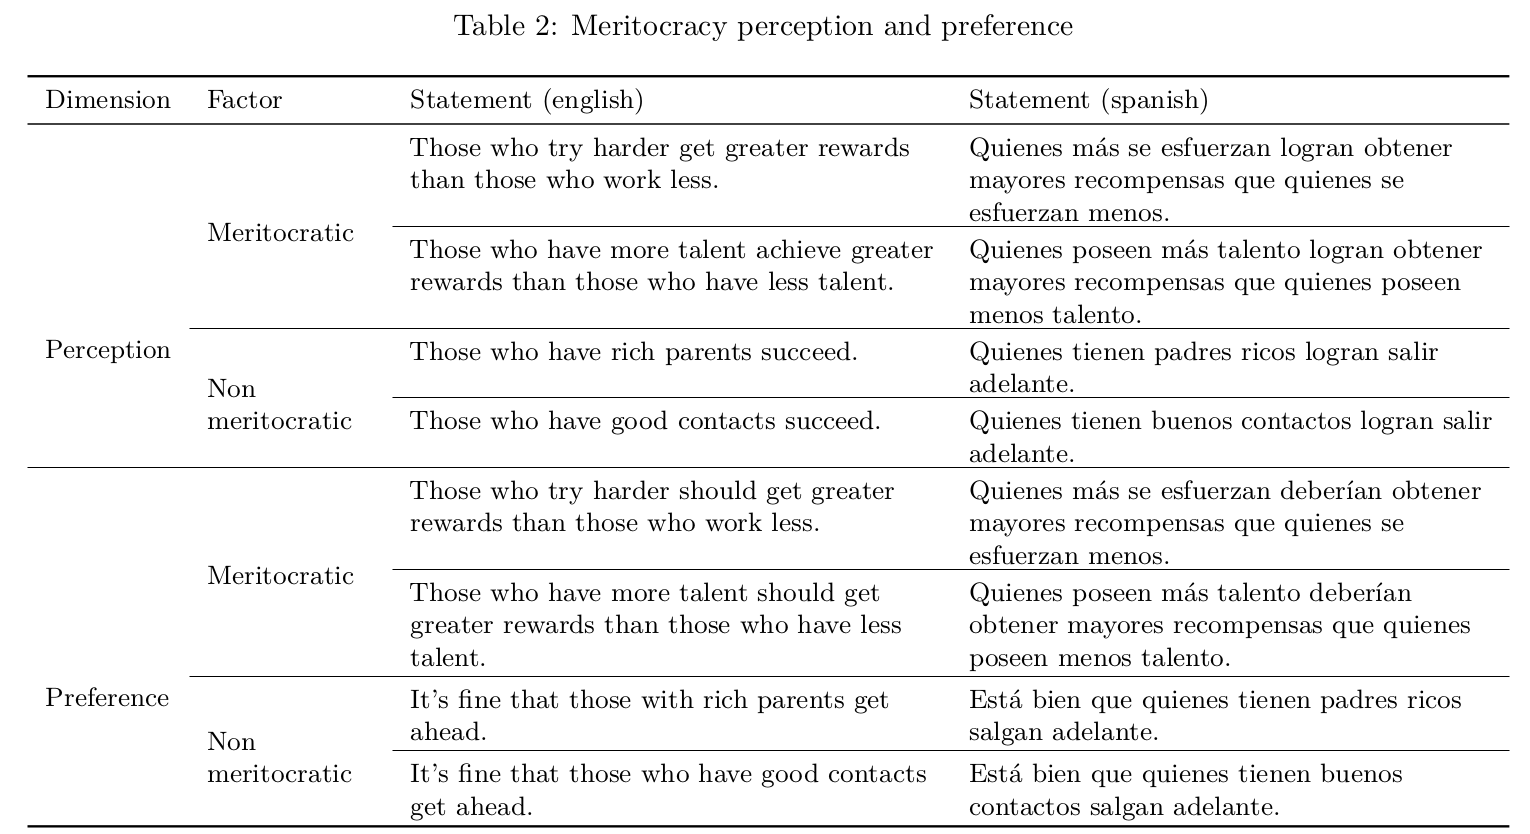
\includegraphics{../input/images/tabla2.png}

1 XX ojo con esta imagen, titularla en el documento, no en la imagen
misma

\hypertarget{administration-sets}{%
\subsection{Administration sets}\label{administration-sets}}

With the objective of evaluating the effect of the order of the
indicators, the respondents (\emph{n = 2141}) were randomly divided into
three groups as explained in \textbf{Diagram 1}. The scale was presented
to the first group (\emph{n = 712}) in the order that appears in Table
2, in such a way that the items of the same factor are found together.
The second group (\emph{n = 717})was presented with the scale with the
items of the same factor separated from each other, in such a way that
they were consulted at the same time for their perceptions and
preferences of a particular topic (e.g.~distribution according to
effort). Finally, in the third group (\emph{n = 712}) the items were
completely randomized.

2 XX agregar número de sujetos por grupo

3 XX referenciar y titular figuras y tablas compatible con html/pdf

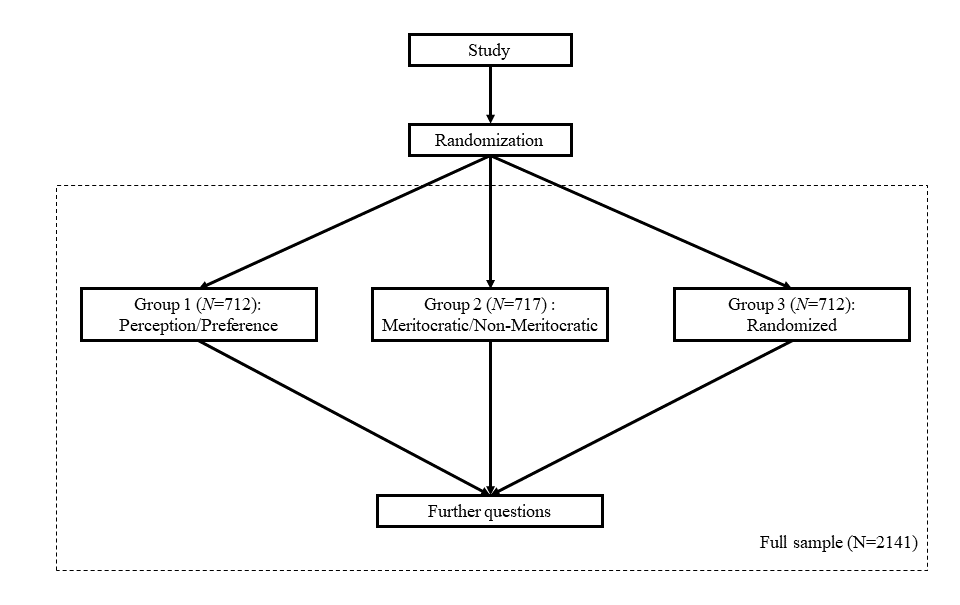
\includegraphics{../input/images/app_mod.png}

\hypertarget{methods}{%
\subsection{Methods}\label{methods}}

For testing the scale's underlying constructs we estimate confirmatory
factor analysis models (CFA). The model estimates one factor for each
dimension, as represented in the following figure:

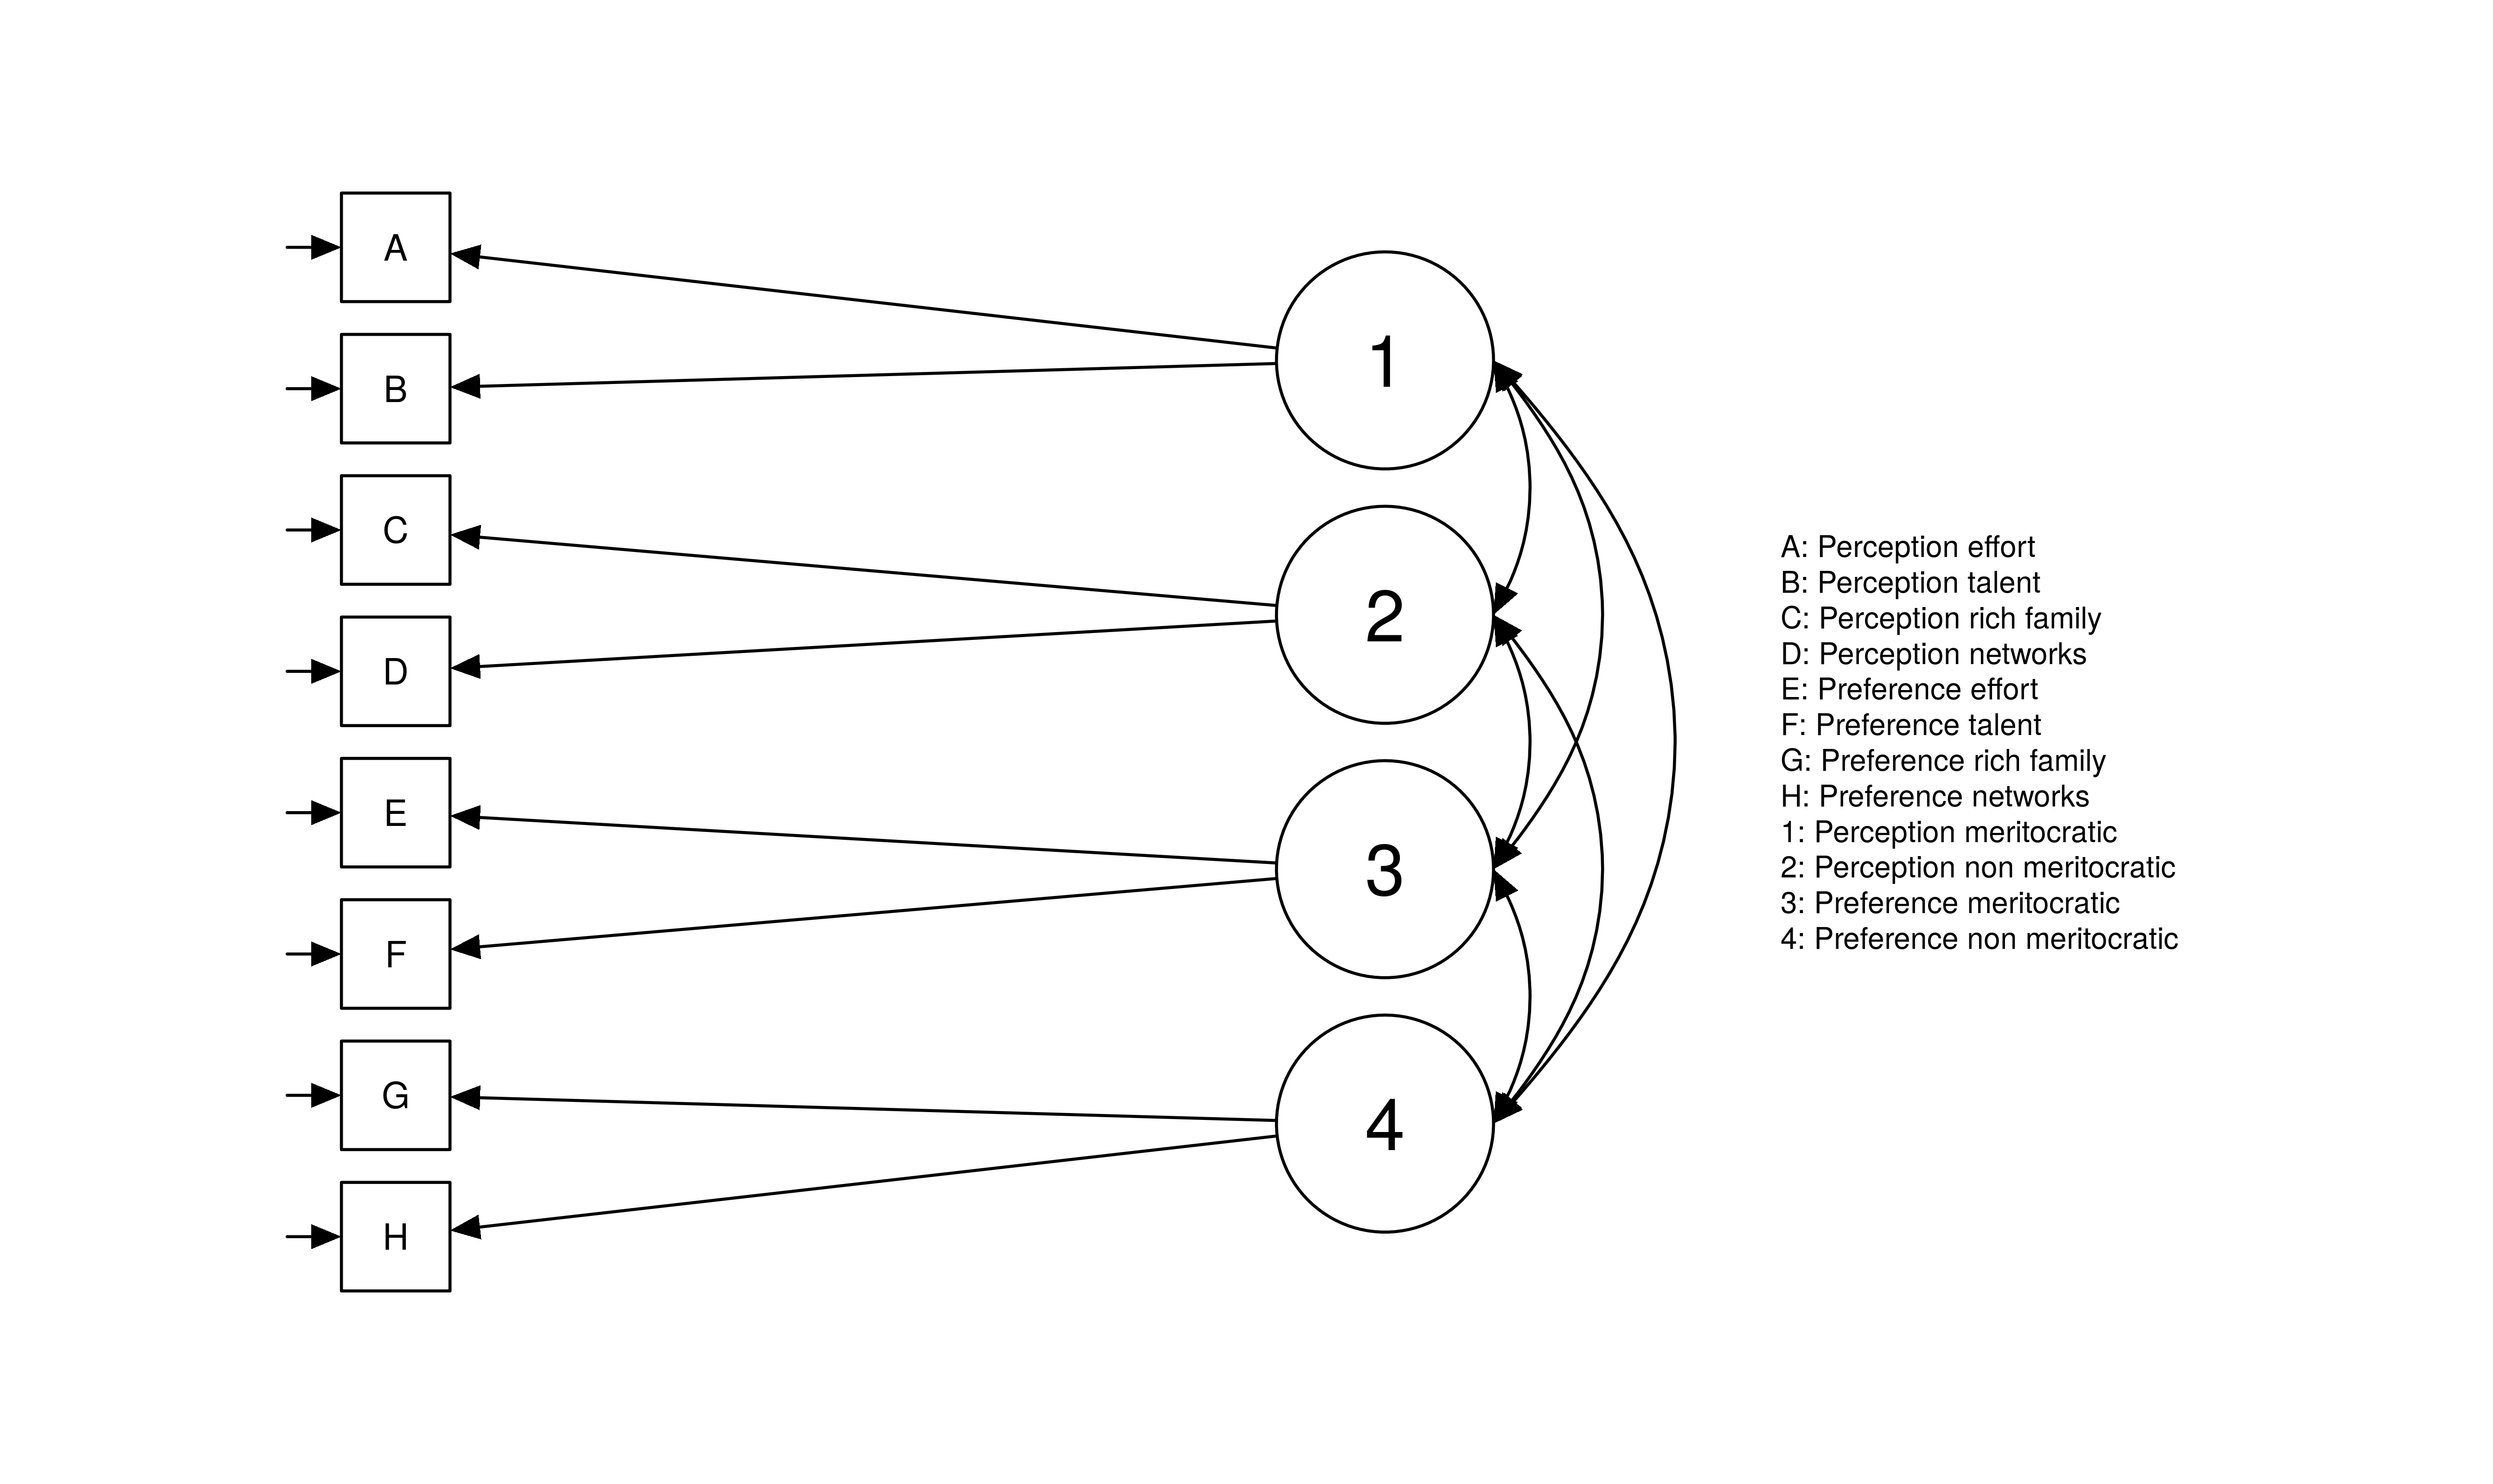
\includegraphics{../output/images/meas01.png}

CFA was conducted using the \texttt{lavaan} package (version 0.6-3;
Rosseel, 2020) with diagonally weighted least squares (DWLS) estimation
due to the items' ordinal level of measurement (Kline, 2016; Rosseel,
2020). As recommended by Brown (2008), we assessed model fit by jointly
considering the comparative fit index and Tucker-Lewis Index (CFI and
TLI; acceptable fit \textgreater{} 0.95), Root of the average squared
residual approximation (RMSEA; acceptable fit \textless{} 0.08),
Chi-square: (p-value; acceptable fit \textgreater{} 0.05, and Chi-square
ratio:\textgreater{} 3).

\hypertarget{results}{%
\section{Results}\label{results}}

\hypertarget{descriptive-analysis}{%
\subsection{Descriptive analysis}\label{descriptive-analysis}}

4 XX producir tabla y llamar directamente desde la fuente o como imagen
{[}\textbf{Pendiente}{]} 5 XX Agregar gráficos de frecuencia , puede ser
tipo trellis 2 x 4, arriba percepción abajo preferencias; la idea es
generar un input más claro para la siguiente idea:

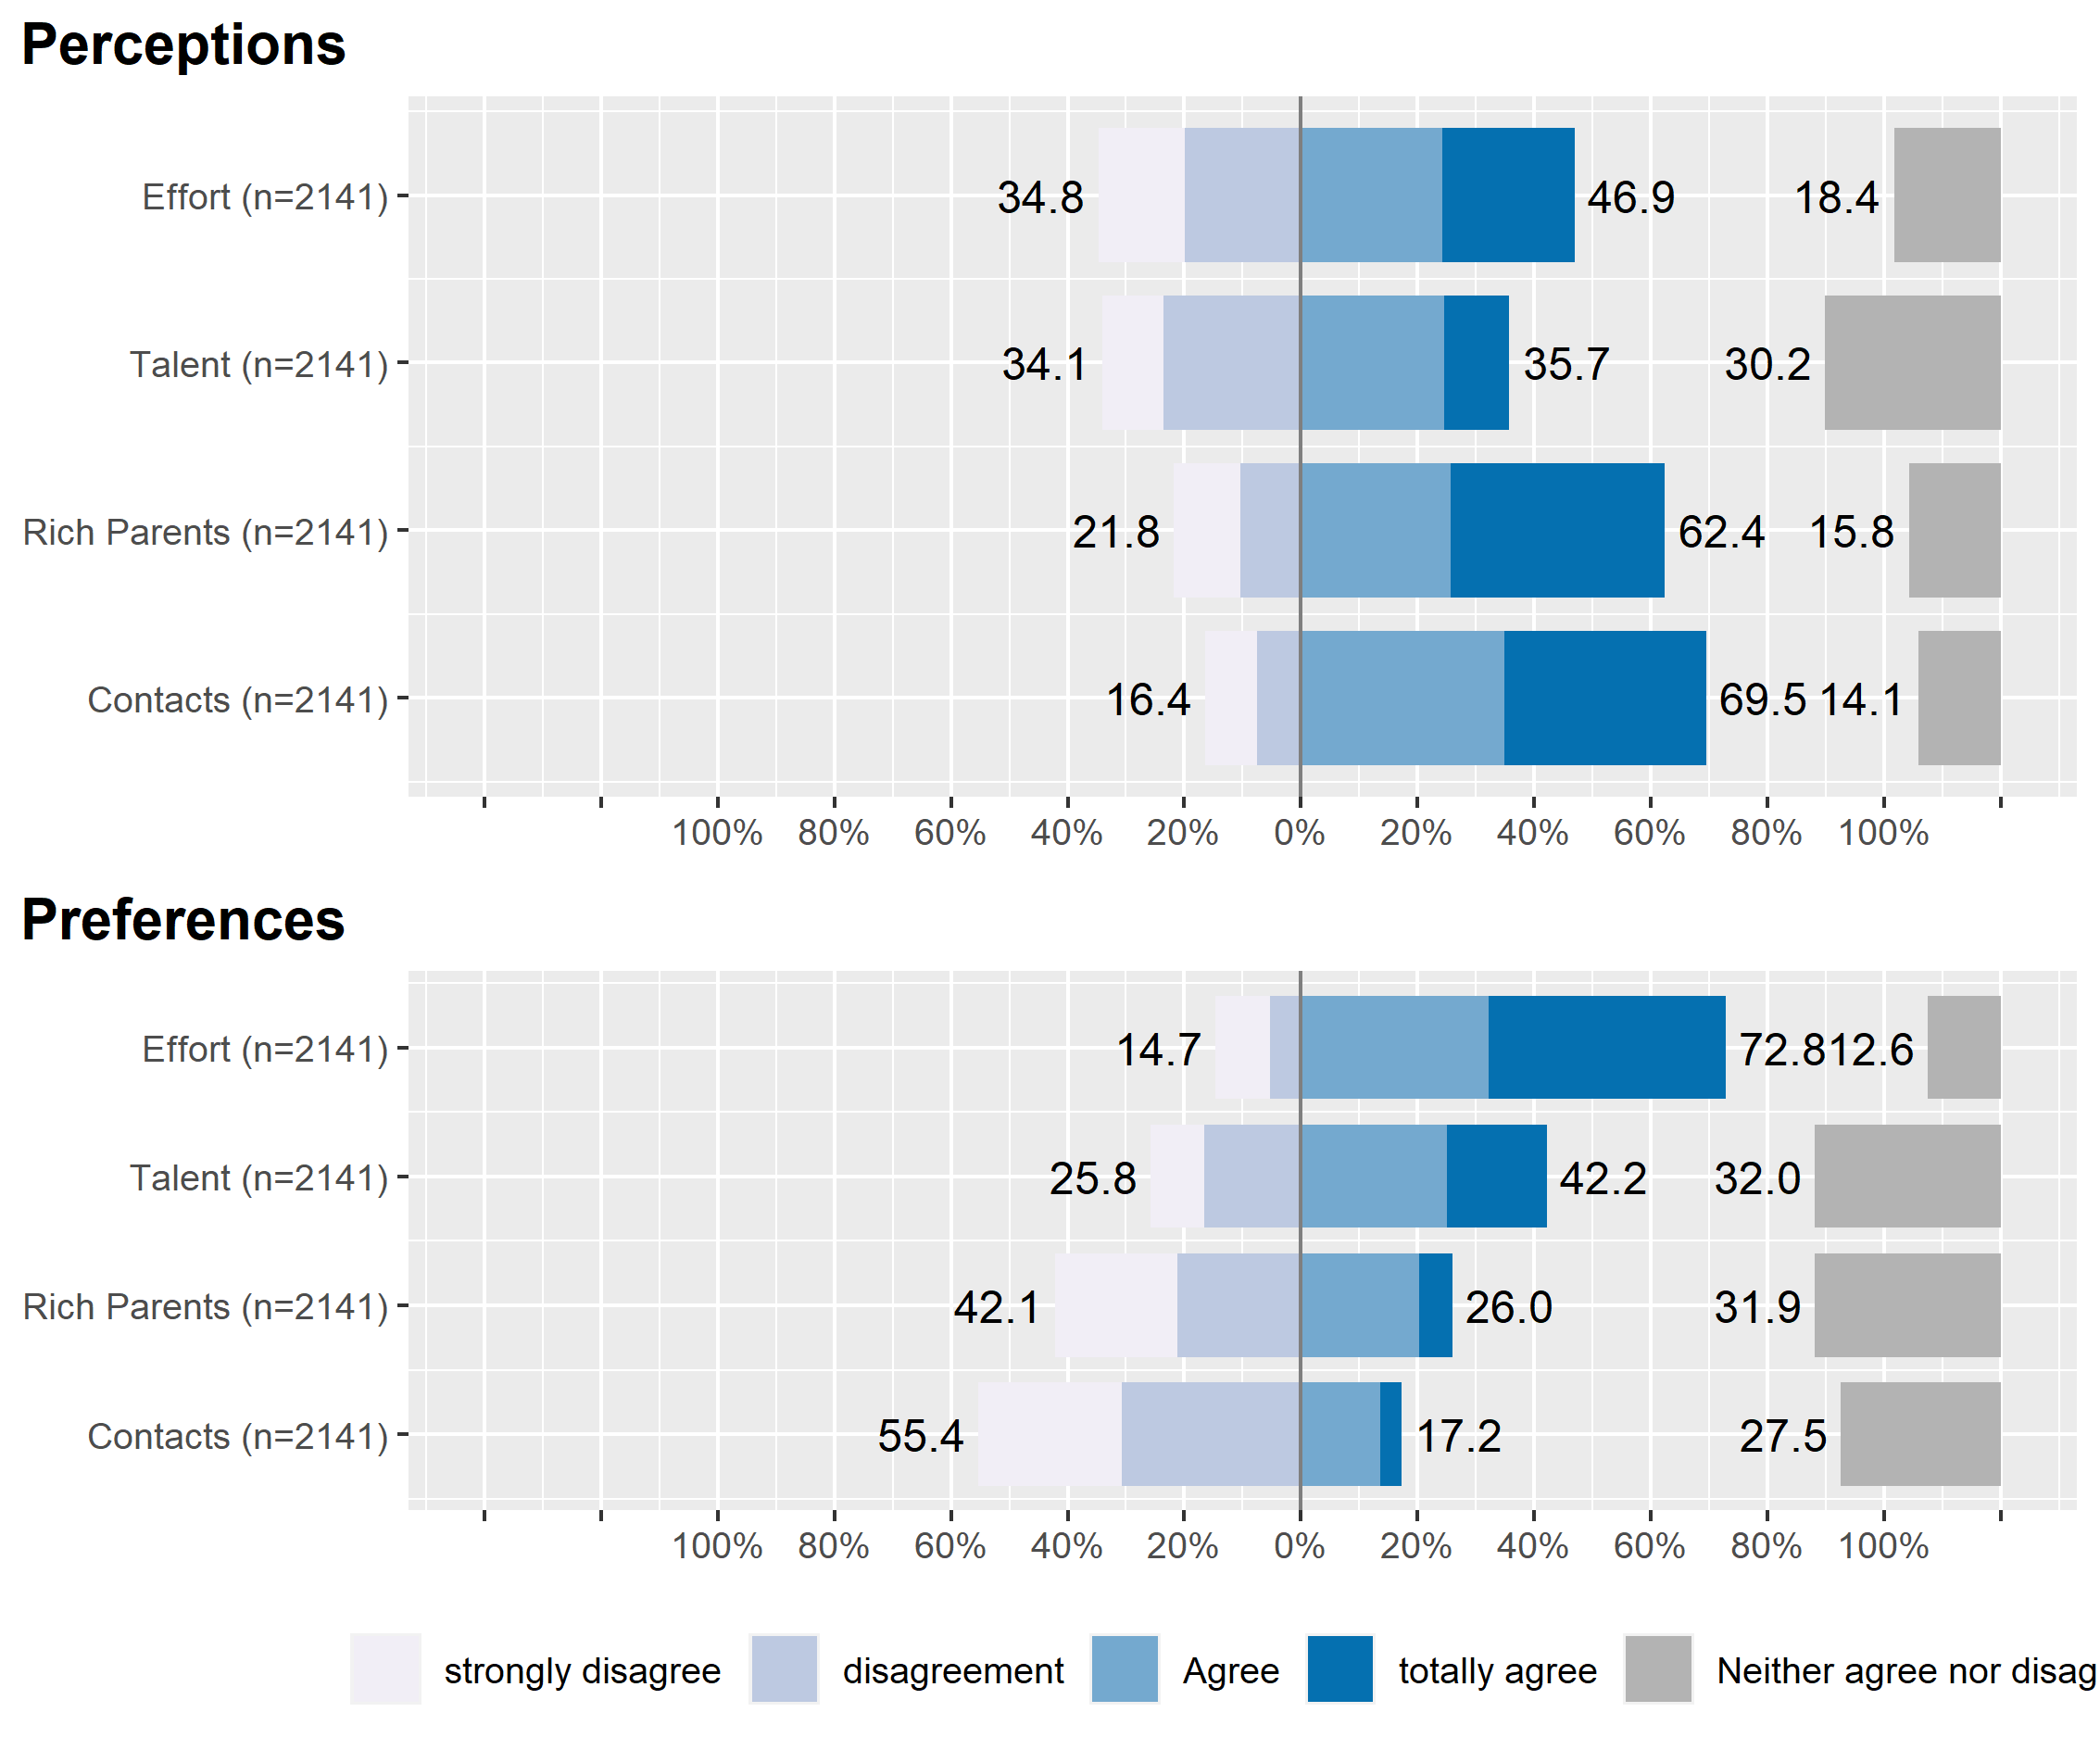
\includegraphics{../output/images/plotlikert.png}

En general se observa que hay una mayor percepción de aspectos no
meritocráticos que meritocráticos, mientras que en el caso de
preferencias ocurre lo opuesto. En cuanto a las preferencias, llama la
atención el rol preponderante del esfuerzo por sobre el talento.

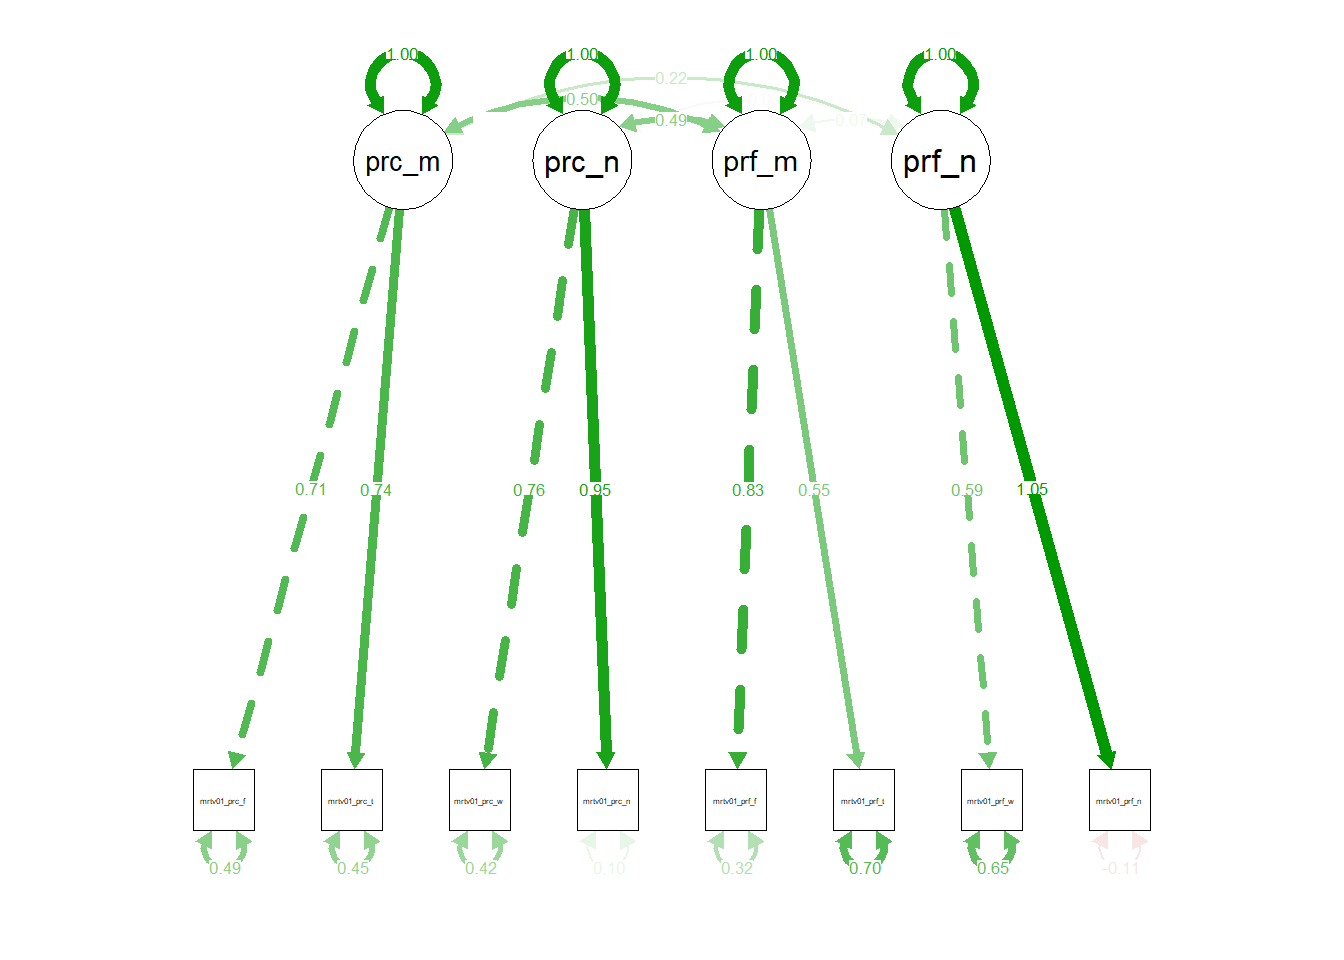
\includegraphics{paper_files/figure-latex/unnamed-chunk-3-1.pdf}

6 - XX Sobre tablas en general, entonces: - dejar tabla de descriptivos
que ahora aparece junto a la de correlaciones {[}\emph{Pendiente} {]} -
agregar gráficos (listo) - reemplazar tabla de correlaciones por un
corrplot, creo que se aprecia más claramente el sentido de las
asociaciones (listo)

\hypertarget{models-estimation}{%
\subsection{Models estimation}\label{models-estimation}}

7 XX En tabla de cargas factoriales, los fit aparecen corridos hacia la
izquierda {[}\textbf{Pendiente}{]}

En una primera instancia se probó el ajuste del modelo con tres
distintos órdenes de los ítems, los cuales fueron aplicados a un tercio
de la muestra de la primera ola cada uno. El primer orden de los ítems
corresponde al orden de de la tabla 2, en el que primero se pregunta a
los encuestados por todas las percepciones y después por todas las
preferencias, en el segundo orden se les pregunta seguidamente por
percepciones y preferencias respecto a un mismo tema, por ejemplo, al
papel del esfuerzo, y en el tercero, los ítems aparecen de manera
aleatoria.

Todos los modelos independiente de los órdenes obtuvieron un ajuste
adecuado. con CFI superiores a .95 y RMSEA inferiores a .8, por
contraparte ni un modelo logró un chi-square no significativo, aunque
tanto el modelo aleatorio como el primero obtuvieron un adecuado
chi-square ratio menor a 3. El primero de los órdenes fue el que obtuvo
mejor ajuste (CFI=0.998, TLI= 0.995,RMSEA=0.037, x2(df=14)=28,03, p =
0.014), seguido por el orden aleatorio de los ítems (CFI=0.992,
TLI=0.984,RMSEA=0.051, x2(df=14)=39.09, p \textless{} 0.001). Por su
parte, la escala ordenada por temáticas parece generar un efecto framing
en el cual la relación entre las percepciones y las preferencias parecen
sobreestimadas, afectando de esta manera el ajuste (CFI=0.984,
TLI=0.968,RMSEA=.071, x2(df=14)=64.156, p \textless{} 0.001).

8 XX explicar mejor lo que viene: invarianza de qué y por qué se
realiza.

Si bien todas las pruebas obtuvieron indicadores relativamente
adecuados, las diferencias mencionadas entre los ajustes de los modelos
según orden son estadísticamente significativas, lo cual fue evaluado a
partir de un análisis de invarianza. Se concluye que entre los tres
órdenes no existe invarianza configuracional, es decir, no poseen la
misma dimensionalidad y por ello no ajustan igualmente al modelo teórico
({\textbf{???}}). Esto se debe al efecto producido por la aparición
conjunta de los ítems de un mismo factor en el orden 1, lo cual aumenta
el ajuste del modelo. Además, en el orden 2, al preguntarse seguidamente
por la percepción y la preferencia en torno al mismo indicador, aumentan
las relaciones cruzadas disminuyendo el ajuste del modelo. De modo
coherente, el modelo aleatorio presentó un ajuste intermedio entre el
orden 1 y el orden 2.

EL modelo teórico propuesto de cuatro factores ajustó, como se observa
en la tabla 4, mejor que el modelo de contraste de 1 factor. El modelo
teórico ajustó de manera relativamente adecuada, pues muestra
indicadores óptimos para CFI= 0.987, TLI = 0.975 y RMSEA=.041, aunque
posee indicadores deficientes para la prueba x2(df=14)=67.6,
p-value=.000. Para evaluar posibles mejoras de la escala, se analizaron
las relaciones propuestas por los índices de modificación. Estos indican
la existencia de dos cargas cruzadas no especificadas. Cuando se generó
un modelo siguiendo estas recomendaciones, hubo una mejora considerable
del modelo, aunque el nuevo modelo tampoco obtuvo un X2 ratio menor a 3
y obtuvo cargas factoriales muy bajas (cargas)\textless{} 0.15, por lo
tanto, siguiendo las recomendación de Brown (2006) de solo aceptar las
propuesta de los índices de modificación cuando se posee teoria y
evidencia sólida, se ha decidido no incorporar estos parámetros al
modelo.

\begin{itemize}
\tightlist
\item
  agregar cuáles fueron las cargas sugeridas.
\end{itemize}

\hypertarget{conclusiuxf3n}{%
\section{Conclusión}\label{conclusiuxf3n}}

Considerando la ventaja del orden, respecto aleatorio despeja la
posibilidad del efecto framing, es decir, de que el resultado del modelo
se deba al orden de las preguntas, se ha decidido seguir utilizando el
orden 3.

\hypertarget{conclusiones}{%
\section{Conclusiones}\label{conclusiones}}

uso conjunto percepciones-preferencias

\hypertarget{anexos}{%
\section{Anexos}\label{anexos}}

\hypertarget{bibliografuxeda}{%
\section*{Bibliografía}\label{bibliografuxeda}}
\addcontentsline{toc}{section}{Bibliografía}

\hypertarget{refs}{}
\leavevmode\hypertarget{ref-AielloNewevidencefirmuniversity2019}{}%
Aiello, Francesco, Paola Cardamone, and Valeria Pupo. 2019. ``New
Evidence on the Firm-University Linkages in Europe. The Role of
Meritocratic Management Practices.'' \emph{International Review of
Applied Economics} 33 (6): 813--28.
\url{https://doi.org/10.1080/02692171.2019.1608917}.

\leavevmode\hypertarget{ref-alesina_Fairness_2005}{}%
Alesina, A., and G. Angeletos. 2005. ``Fairness and Redistribution.''
\emph{American Economic Review}, 960--80.

\leavevmode\hypertarget{ref-arrow_meritocracy_2000}{}%
Arrow, Kenneth J., Samuel Bowles, and Steven N. Durlauf, eds. 2000.
\emph{Meritocracy and Economic Inequality}. Princeton, N.J: Princeton
University Press.

\leavevmode\hypertarget{ref-Bay-ChengTrackingHomoOeconomicus2015}{}%
Bay-Cheng, Laina Y., Caroline C. Fitz, Natalie M. Alizaga, and Alyssa N.
Zucker. 2015. ``Tracking Homo Oeconomicus: Development of the Neoliberal
Beliefs Inventory.'' \emph{Journal of Social and Political Psychology} 3
(1): 71--88. \url{https://doi.org/10.5964/jspp.v3i1.366}.

\leavevmode\hypertarget{ref-breenClassInequalityMeritocracy1999}{}%
Breen, Richard, and John H. Goldthorpe. 1999. ``Class Inequality and
Meritocracy: A Critique of Saunders and an Alternative Analysis1.''
\emph{The British Journal of Sociology} 50 (1): 1--27.
\url{https://doi.org/10.1111/j.1468-4446.1999.00001.x}.

\leavevmode\hypertarget{ref-BubakPerceptionsmeritocracynote2019}{}%
Bubak, Oldrich. 2019. ``Perceptions of Meritocracy: A Note on China.''
\emph{Asian Journal of Comparative Politics} 4 (2): 192--209.
\url{https://doi.org/10.1177/2057891118806065}.

\leavevmode\hypertarget{ref-davey_preference_1999}{}%
Davey, L. M., D. R. Bobocel, L. S. Son Hing, and M. P. Zanna. 1999.
``Preference for the Merit Principle Scale: An Individual Difference
Measure of Distributive Justice Preferences.'' \emph{Social Justice
Research} 12 (3): 223--40.

\leavevmode\hypertarget{ref-dimick_Models_2018}{}%
Dimick, Matthew, David Rueda, and Daniel Stegmueller. 2018. ``Models of
Other-Regarding Preferences, Inequality, and Redistribution.''
\emph{Annual Review of Political Science} 21 (1): 441--60.
\url{https://doi.org/10.1146/annurev-polisci-091515-030034}.

\leavevmode\hypertarget{ref-Duru-BellatWhoMeritocracyIndividual2012b}{}%
Duru-Bellat, Marie, and Elise Tenret. 2012a. ``Who's for Meritocracy?
Individual and Contextual Variations in the Faith.'' \emph{Comparative
Education Review} 56 (2): 223--47. \url{https://doi.org/10.1086/661290}.

\leavevmode\hypertarget{ref-duru-bellat_whos_2012}{}%
---------. 2012b. ``Who's for Meritocracy? Individual and Contextual
Variations in the Faith.'' \emph{Comparative Education Review} 56 (2):
223--47. \url{https://doi.org/10.1086/661290}.

\leavevmode\hypertarget{ref-GenerettStoriesWeTell2020}{}%
Generett, Gretchen Givens, and Amy M. Olson. 2020. ``The Stories We
Tell: How Merit Narratives Undermine Success for Urban Youth.''
\emph{Urban Education} 55 (3): 394--423.
\url{https://doi.org/10.1177/0042085918817342}.

\leavevmode\hypertarget{ref-GirerdNeoliberalismIdeologicalBarrier2020}{}%
Girerd, Lola, and Virginie Bonnot. 2020. ``Neoliberalism: An Ideological
Barrier to Feminist Identification and Collective Action.'' \emph{Social
Justice Research} 33 (1): 81--109.
\url{https://doi.org/10.1007/s11211-020-00347-8}.

\leavevmode\hypertarget{ref-goldthorpe_myth_2003}{}%
Goldthorpe, John. 2003. ``The Myth of Education-Based Meritocracy.''
\emph{New Economy} 10 (4): 234--39.
\url{https://doi.org/10.1046/j.1468-0041.2003.00324.x}.

\leavevmode\hypertarget{ref-hadjar_meritokratie_2008}{}%
Hadjar, Andreas. 2008. \emph{Meritokratie Als Legitimationsprinzip}.
Wiesbaden: VS Verlag.

\leavevmode\hypertarget{ref-kunovich_systems_2007}{}%
Kunovich, Sheri, and Kazimierz M. Slomczynski. 2007. ``Systems of
Distribution and a Sense of Equity: A Multilevel Analysis of
Meritocratic Attitudes in Post-Industrial Societies.'' \emph{European
Sociological Review} 23 (5): 649--63.
\url{https://doi.org/10.1093/esr/jcm026}.

\leavevmode\hypertarget{ref-landWeSatTable2006}{}%
Land, Hilary. 2006. ``We Sat down at the Table of Privilege and
Complained About the Food \textsuperscript{1}.'' \emph{The Political
Quarterly} 77 (s1): 45--60.
\url{https://doi.org/10.1111/j.1467-923X.2006.00780.x}.

\leavevmode\hypertarget{ref-MadeiraPrimesConsequencesSystematic2019}{}%
Madeira, Ana Filipa, Rui Costa-Lopes, John F. Dovidio, Gonçalo Freitas,
and Mafalda F. Mascarenhas. 2019. ``Primes and Consequences: A
Systematic Review of Meritocracy in Intergroup Relations.''
\emph{Frontiers in Psychology} 10 (September).
\url{https://doi.org/10.3389/fpsyg.2019.02007}.

\leavevmode\hypertarget{ref-MaitnerEmotionalreactionsunequal2015}{}%
Maitner, Angela T. 2015. ``Emotional Reactions to Unequal Payment: The
Impact of Meritocratic Ideology and Salary Negotiability.'' \emph{Group
Processes \& Intergroup Relations} 18 (2): 153--72.
\url{https://doi.org/10.1177/1368430214542255}.

\leavevmode\hypertarget{ref-MajorPerceiveddiscriminationworldview2007}{}%
Major, Brenda, Cheryl R. Kaiser, Laurie T. O'Brien, and Shannon K.
McCoy. 2007. ``Perceived Discrimination as Worldview Threat or Worldview
Confirmation: Implications for Self-Esteem.'' \emph{Journal of
Personality and Social Psychology} 92 (6): 1068--86.
\url{https://doi.org/10.1037/0022-3514.92.6.1068}.

\leavevmode\hypertarget{ref-markovits_Meritocracy_2019}{}%
Markovits, Daniel. 2019. \emph{The Meritocracy Trap: How America's
Foundational Myth Feeds Inequality, Dismantles the Middle Class, and
Devours the Elite}. New York: Penguin Press.

\leavevmode\hypertarget{ref-Meredithsocietydivisibleblessed2020}{}%
Meredith, Stephen. 2020. ``A `Society \ldots{} Divisible into the
Blessed and the Unblessed': Michael Young and Meritocracy in Postwar
Britain: Michael Young and Meritocracy in Postwar Britain.'' \emph{The
Political Quarterly}, March.
\url{https://doi.org/10.1111/1467-923X.12837}.

\leavevmode\hypertarget{ref-MijsParadoxInequalityIncome2019b}{}%
Mijs, Jonathan J B. 2019a. ``The Paradox of Inequality: Income
Inequality and Belief in Meritocracy Go Hand in Hand.''
\emph{Socio-Economic Review}, January.
\url{https://doi.org/10.1093/ser/mwy051}.

\leavevmode\hypertarget{ref-mijs_paradox_2019}{}%
---------. 2019b. ``The Paradox of Inequality: Income Inequality and
Belief in Meritocracy Go Hand in Hand.'' \emph{Socio-Economic Review},
January. \url{https://doi.org/10.1093/ser/mwy051}.

\leavevmode\hypertarget{ref-newman_false_2015}{}%
Newman, Benjamin J., Christopher D. Johnston, and Patrick L. Lown. 2015.
``False Consciousness or Class Awareness? Local Income Inequality,
Personal Economic Position, and Belief in American Meritocracy.''
\emph{American Journal of Political Science} 59 (2): 326--40.
\url{https://doi.org/10.1111/ajps.12153}.

\leavevmode\hypertarget{ref-OwensENGINESSOCIALMOBILITY2020}{}%
Owens, John, and Tania de St Croix. 2020. ``ENGINES OF SOCIAL MOBILITY?
NAVIGATING MERITOCRATIC EDUCATION DISCOURSE IN AN UNEQUAL SOCIETY.''
\emph{British Journal of Educational Studies}, January, 1--21.
\url{https://doi.org/10.1080/00071005.2019.1708863}.

\leavevmode\hypertarget{ref-PerezAdvancingcareersmerit2020}{}%
Pérez, Andrés, and Ida Sabelis. 2020. ``Advancing Careers Through
`Merit': A Rationalized-Sensemaking Narrative in Hierarchical
Organizations.'' \emph{Culture and Organization} 26 (4): 315--32.
\url{https://doi.org/10.1080/14759551.2019.1601723}.

\leavevmode\hypertarget{ref-PikettyCapitalTwentyFirstCentury2014b}{}%
Piketty, Thomas. 2014. \emph{Capital in the Twenty-First Century}.
Translated by Arthur Goldhammer. Cambridge Massachusetts: The Belknap
Press of Harvard University Press.

\leavevmode\hypertarget{ref-PremingerMeritocracyserviceethnocracy2020}{}%
Preminger, Jonathan. 2020. ``Meritocracy in the Service of Ethnocracy.''
\emph{Citizenship Studies} 24 (2): 247--63.
\url{https://doi.org/10.1080/13621025.2020.1720604}.

\leavevmode\hypertarget{ref-ReayPerilsPenaltiesMeritocracy2020}{}%
Reay, Diane. 2020. ``The Perils and Penalties of Meritocracy:
Sanctioning Inequalities and Legitimating Prejudice.'' \emph{The
Political Quarterly}, March, 1467--923X.12829.
\url{https://doi.org/10.1111/1467-923X.12829}.

\leavevmode\hypertarget{ref-ReynoldsPerceptionsMeritocracyLand2014b}{}%
Reynolds, Jeremy, and He Xian. 2014a. ``Perceptions of Meritocracy in
the Land of Opportunity.'' \emph{Research in Social Stratification and
Mobility} 36 (June): 121--37.
\url{https://doi.org/10.1016/j.rssm.2014.03.001}.

\leavevmode\hypertarget{ref-reynolds_perceptions_2014}{}%
---------. 2014b. ``Perceptions of Meritocracy in the Land of
Opportunity.'' \emph{Research in Social Stratification and Mobility} 36
(June): 121--37. \url{https://doi.org/10.1016/j.rssm.2014.03.001}.

\leavevmode\hypertarget{ref-saundersMightBritainBe1995}{}%
Saunders, Peter. 1995. ``Might Britain Be a Meritocracy?''
\emph{Sociology} 29 (1): 23--41.
\url{https://doi.org/10.1177/0038038595029001003}.

\leavevmode\hypertarget{ref-schroder_Income_2017}{}%
Schröder, Martin. 2017. ``Is Income Inequality Related to Tolerance for
Inequality?'' \emph{Social Justice Research} 30 (1): 23--47.
\url{https://doi.org/10.1007/s11211-016-0276-8}.

\leavevmode\hypertarget{ref-son_hing_merit_2011-1}{}%
Son Hing, Leanne S., D. Ramona, Mark P. Zanna, Donna M. Garcia,
Stephanie S. Gee, and Katie Orazietti. 2011. ``The Merit of
Meritocracy.'' \emph{Journal of Personality and Social Psychology} 101
(3): 433--50. \url{https://doi.org/10.1037/a0024618}.

\leavevmode\hypertarget{ref-TrumpWhenwhyeconomic2020}{}%
Trump, Kris-Stella. 2020. ``When and Why Is Economic Inequality Seen as
Fair.'' \emph{Current Opinion in Behavioral Sciences} 34 (August):
46--51. \url{https://doi.org/10.1016/j.cobeha.2019.12.001}.

\leavevmode\hypertarget{ref-WitteveenReconsideringmeritocraticpower2020a}{}%
Witteveen, Dirk, and Paul Attewell. 2020. ``Reconsidering the
`Meritocratic Power of a College Degree'.'' \emph{Research in Social
Stratification and Mobility} 66 (April): 100479.
\url{https://doi.org/10.1016/j.rssm.2020.100479}.

\leavevmode\hypertarget{ref-yairMeritocracy2007}{}%
Yair, Gad. 2007. ``Meritocracy.'' In \emph{The Blackwell Encyclopedia of
Sociology}, edited by George Ritzer. Oxford, UK: John Wiley \& Sons,
Ltd. \url{https://doi.org/10.1002/9781405165518.wbeosm082}.

\leavevmode\hypertarget{ref-young_rise_1962}{}%
Young, M. 1962. \emph{The Rise of the Meritocracy}. Baltimore: Penguin
Books.

\leavevmode\hypertarget{ref-youngRiseMeritocracy1994}{}%
Young, Michael Dunlop. 1994. \emph{The Rise of the Meritocracy}. New
Brunswick, N.J., U.S.A: Transaction Publishers.

\end{document}
